\documentclass{article}
\usepackage[a3paper,landscape,margin=.5in]{geometry}
\usepackage[T1]{fontenc}
\usepackage{cmbright}
\usepackage{marvosym}
\usepackage{multicol}

\usepackage{tikz}
\usetikzlibrary{shapes.multipart}
\usetikzlibrary{fit}
\newcommand{\shiftXL}{-11cm}
\newcommand{\shiftXR}{5cm}
\newcommand{\shiftYD}{-6cm}
\newcommand{\shiftYU}{3cm}
\newcommand{\shiftXA}{-4cm}
\newcommand{\shiftXB}{12cm}
\newcommand{\shiftYA}{-4cm}
\newcommand{\shiftYB}{5cm}

\newcommand{\cubewrap}[2]{
\node (WR#1) [draw,rectangle,rounded corners,draw=#2!40,fill=#2!10,fit=(000#1) (100#1) (010#1) (101#1) (111#1)] {};
}
\newcommand{\tikzcube}[9]{
\node (000#1) at (-2,-2) {#2}; % active
\node (100#1) at (2,-2) {#3}; % active continuous
\node (010#1) at (-2,2) {#4}; % active perfect
\node (110#1) at (2,2) {#5}; % active perfect continuous
\node (001#1) at (-1,-1) {#6}; % passive
\node (101#1) at (3,-1) {#7}; % passive continous
\node (011#1) at (-1,3) {#8}; % passive perfect
\node (111#1) at (3,3) {#9}; % passive perfect continuous
\pgfonlayer{cubeskelet}
\draw [opacity=0.3] (000#1) -- (100#1) -- (110#1) -- (010#1);
\draw [opacity=0.3] (001#1) -- (000#1) -- (010#1) -- (011#1);
\draw [opacity=0.3] (101#1) -- (001#1) -- (011#1) -- (111#1);
\draw [opacity=0.3] (100#1) -- (101#1) -- (111#1) -- (110#1);
\endpgfonlayer
}
\pgfdeclarelayer{background}
\pgfdeclarelayer{cubeskelet}
\pgfsetlayers{background,cubeskelet,main}

\begin{document}
\thispagestyle{empty}
\begin{center}
\noindent{\Huge\bfseries Verb Tenses Overview}\\
{\bfseries 64 of them, on a hypercube.}
\vfill
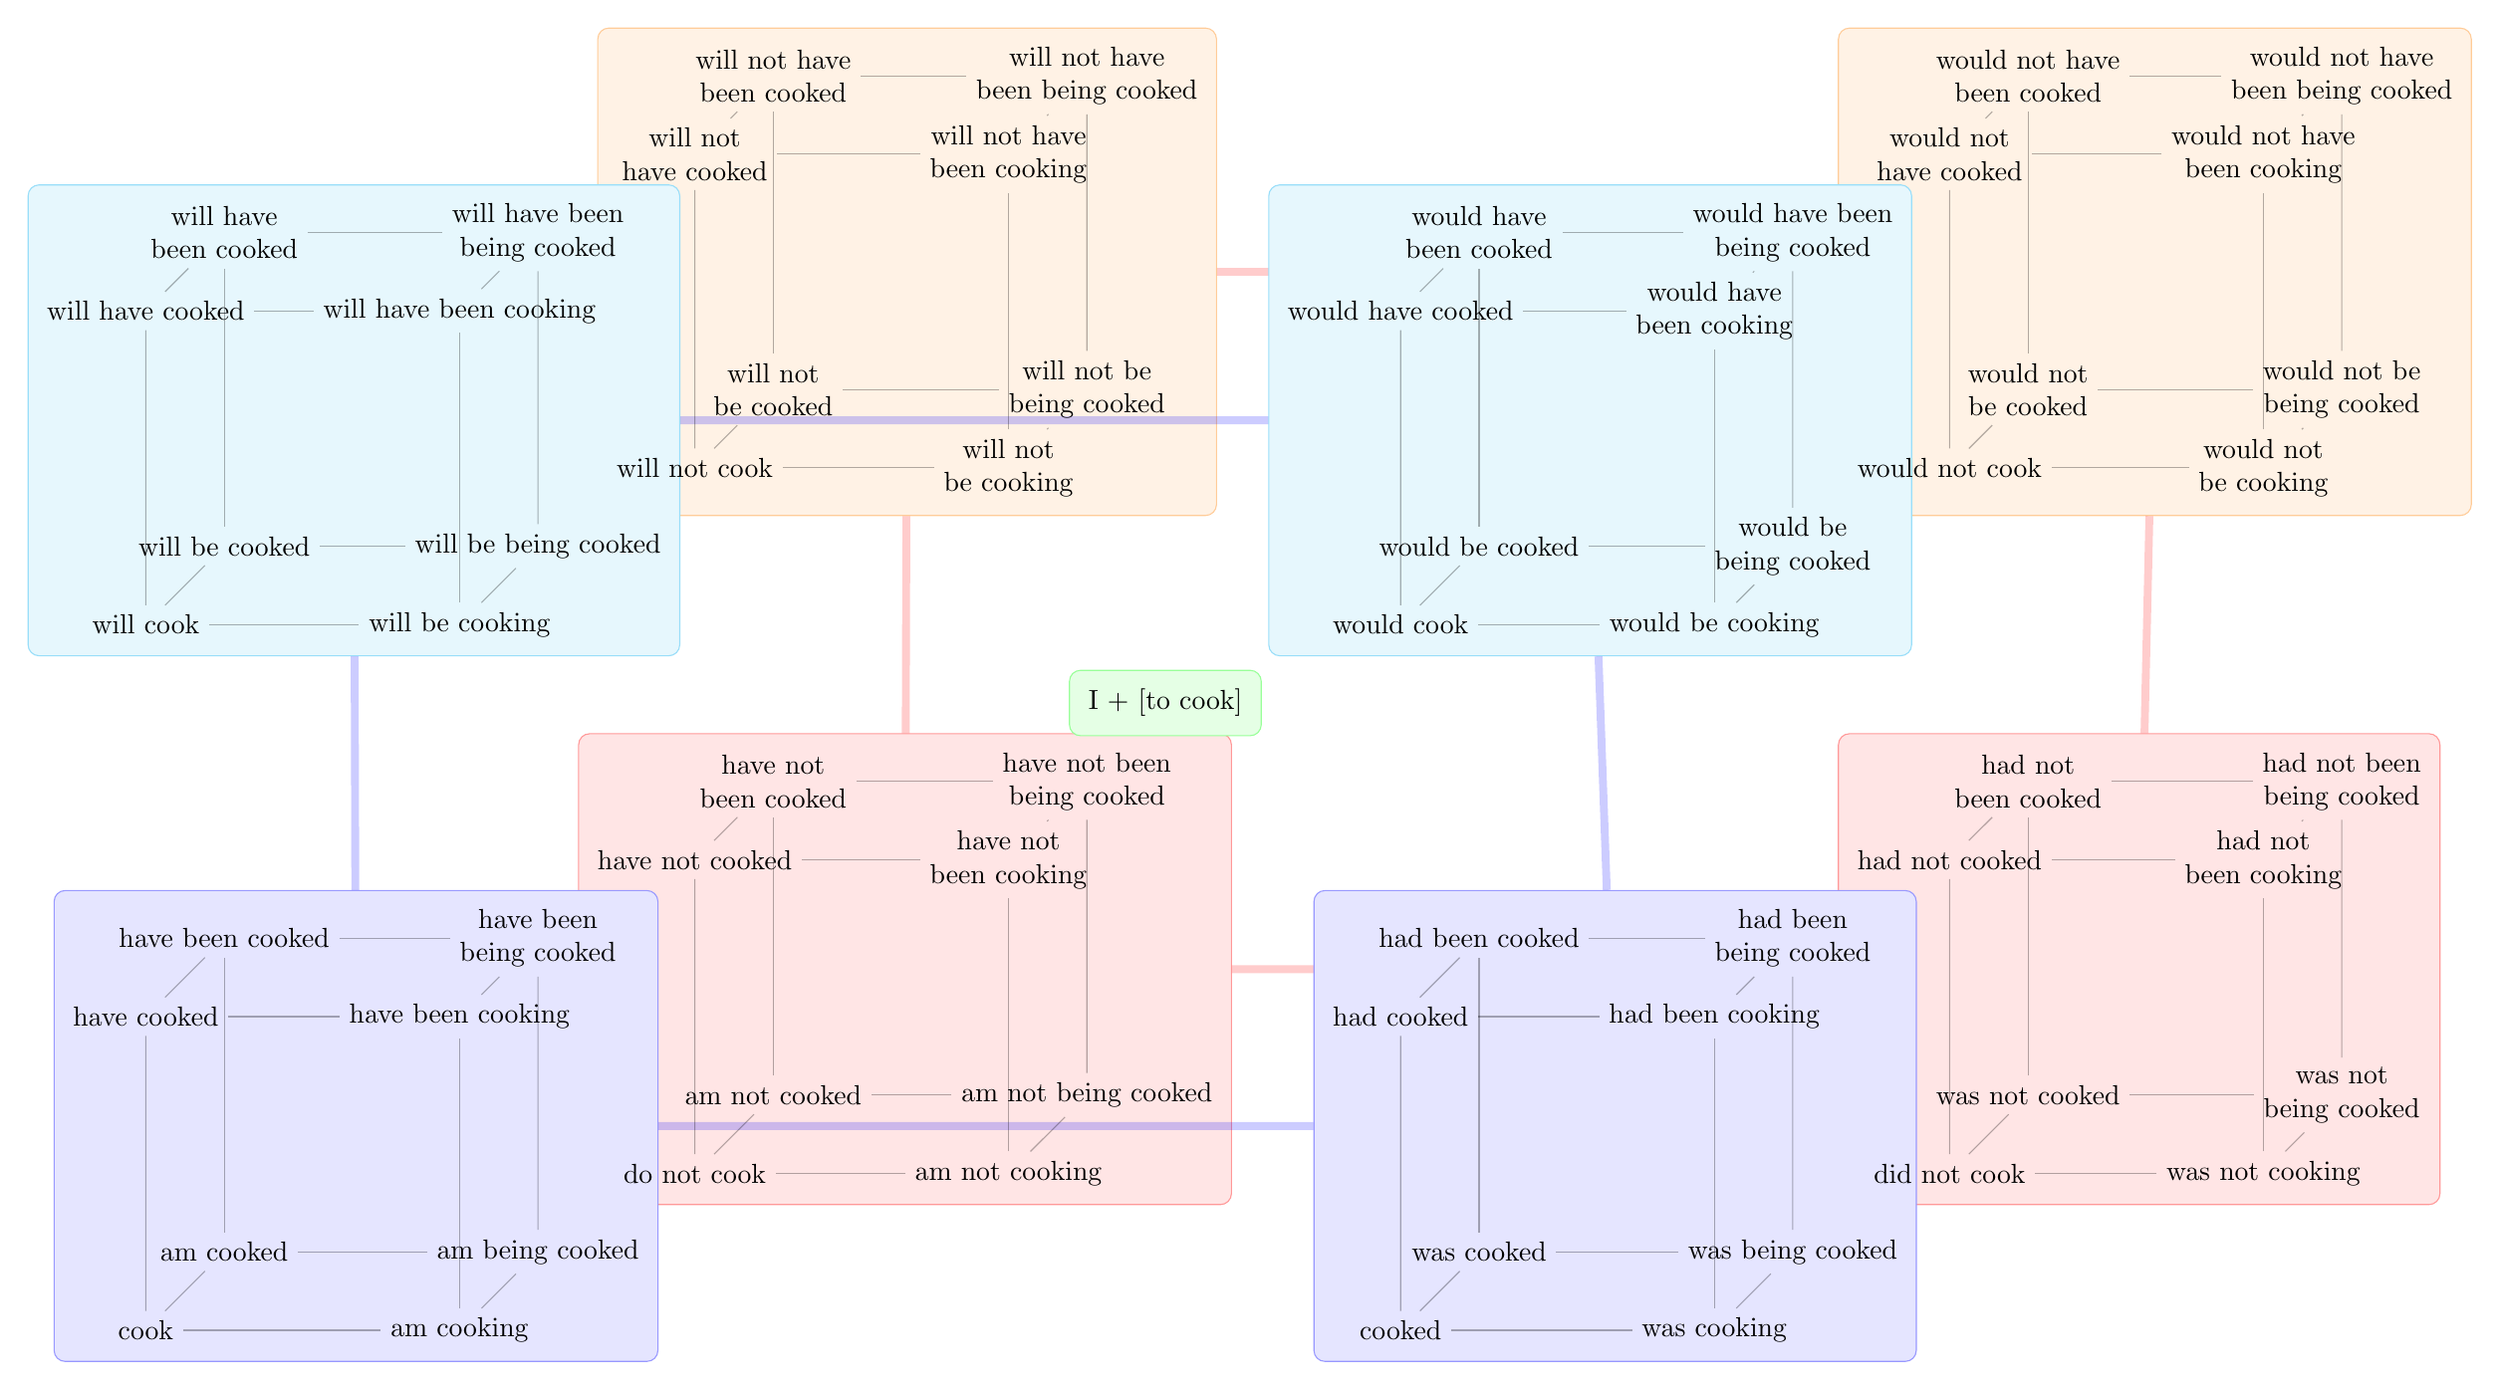
\begin{tikzpicture}[every text node part/.style={align=center}]
\node (inf) at (0,0) {I + [to cook]};
\begin{scope} [xshift=\shiftXL,yshift=\shiftYD]
% present positive
\tikzcube{AAA}{cook}{am cooking}{have cooked}{have been cooking}{am cooked}{am being cooked}{have been cooked}{have been\\being cooked}
\end{scope}
\begin{scope} [xshift=\shiftXR,yshift=\shiftYD]
% past positive
\tikzcube{BAA}{cooked}{was cooking}{had cooked}{had been cooking}{was cooked}{was being cooked}{had been cooked}{had been\\being cooked}
\end{scope}
\begin{scope} [xshift=\shiftXL,yshift=\shiftYU]
% future positive
\tikzcube{ABA}{will cook}{will be cooking}{will have cooked}{will have been cooking}{will be cooked}{will be being cooked}{will have\\been cooked}{will have been\\being cooked}
\end{scope}
\begin{scope} [xshift=\shiftXR,yshift=\shiftYU]
% conditional positive
\tikzcube{BBA}{would cook}{would be cooking}{would have cooked}{would have\\been cooking}{would be cooked}{would be\\being cooked}{would have\\been cooked}{would have been\\being cooked}
\end{scope}
\begin{scope} [xshift=\shiftXA,yshift=\shiftYA]
% present negative
\tikzcube{AAB}{do not cook}{am not cooking}{have not cooked}{have not\\been cooking}{am not cooked}{am not being cooked}{have not\\been cooked}{have not been\\being cooked}
\end{scope}
\begin{scope} [xshift=\shiftXB,yshift=\shiftYA]
% past negative
\tikzcube{BAB}{did not cook}{was not cooking}{had not cooked}{had not\\been cooking}{was not cooked}{was not\\being cooked}{had not\\been cooked}{had not been\\being cooked}
\end{scope}
\begin{scope} [xshift=\shiftXA,yshift=\shiftYB]
% future negative
\tikzcube{ABB}{will not cook}{will not\\be cooking}{will not\\have cooked}{will not have\\been cooking}{will not\\be cooked}{will not be\\being cooked}{will not have\\been cooked}{will not have\\been being cooked}
\end{scope}
\begin{scope} [xshift=\shiftXB,yshift=\shiftYB]
% conditional negative
\tikzcube{BBB}{would not cook}{would not\\be cooking}{would not\\have cooked}{would not have\\been cooking}{would not\\be cooked}{would not be\\being cooked}{would not have\\been cooked}{would not have\\been being cooked}

% big nodes
\pgfonlayer{background}
\cubewrap{AAB}{red};
\cubewrap{BAB}{red};
\cubewrap{ABB}{orange};
\cubewrap{BBB}{orange};
\draw [opacity=0.2,draw=red,line width=1mm] (WRAAB) -- (WRBAB) -- (WRBBB) -- (WRABB) -- (WRAAB);
\node (WRinf) [draw,rectangle,rounded corners,draw=green!40,fill=green!10,fit=(inf)] {};
\cubewrap{AAA}{blue};
\cubewrap{BAA}{blue};
\cubewrap{ABA}{cyan};
\cubewrap{BBA}{cyan};
\draw [opacity=0.2,draw=blue,line width=1mm] (WRAAA) -- (WRBAA) -- (WRBBA) -- (WRABA) -- (WRAAA);
\endpgfonlayer
\end{scope}
\end{tikzpicture}
\vfill
\parbox{44em}{\emph{How to use this?}
Say you want to form a sentence about cooking with ``I'' in subject and some
weird tense.
\begin{multicols}{2}
{\bfseries 1.} Choose the basic tense from the ``big'' cubes:
\begin{itemize}
\item[start] bottom-left (present)
\item[$\rightarrow$] to the past
\item[$\uparrow$] to the future
\item[$\rightarrow\uparrow$] go conditional
\item[$\nearrow$] optionally go negative
\end{itemize}
\columnbreak
{\bfseries 2.} Refine the choice by moving in the smaller cube:
\begin{itemize}
\item[start] bottom left (imperfect active simple)
\item[$\rightarrow$] make the tense continuous
\item[$\uparrow$] make the tense perfect
\item[$\nearrow$] make the tense passive
\end{itemize}

\end{multicols}
}
\end{center}
\end{document}
